% 狄拉克 delta 函数

\pentry{定积分\upref{DefInt}}
在物理中我们经常会遇到一些模型, 如质点和点电荷等, 这类模型使用了极限的思想(如令体积趋于无穷小). 如果考察质点的密度或点电荷的电荷密度, 将得到无穷大, 然而将其密度(电荷密度)在空间中积分却又能得到有限的质量与电荷. 为了描述这样的密度(电荷密度)分布, 我们引入狄拉克 $\delta$ 函数.

\subsection{一维情况}

\begin{figure}[ht]
\centering
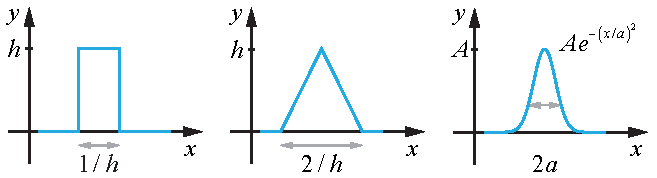
\includegraphics[width=11cm]{./figures/Delta1.pdf}
\caption{$\delta(x - x_0)$ 的几个例子} \label{Delta_fig1}
\end{figure}

我们来考虑一个函数(\autoref{Delta_fig1} 左)
\begin{equation}
f(x) = \leftgroup{
&h &\quad & \qty( \abs{x - x_0} \les \frac{1}{2h} )\\
&0 &          & \qty( \abs{x - x_0} > \frac{1}{2h} )
}\end{equation}
其中 $h, x_0$ 是常数. 由函数图像易得函数曲线下面的面积为 $\int_{-\infty}^{+\infty} f(x) \dd{x} = 1$. 现在我们令 $h \to 0$, 长方形的高将趋于无穷大, 宽将趋于零, 而定积分结果不变.

我们定义\bb{狄拉克 $\delta$ 函数}\footnote{严格来说, 这并不是一个数学上的函数, 但在物理中却经常出现.} $\delta(x)$ 为满足以下两个性质的函数
\begin{align}
&\delta(x) = \leftgroup{
+&\infty &\quad& (x = 0)\\
&0 && (x \ne 0)}\\
&\int_{-\infty}^{+\infty} \delta(x) \dd{x} = 1
\end{align}
这样, 上面的 $f(x)$ 就可以表示为 $\delta(x - x_0)$. 当然, 我们还可以选取其他含有参数的 $f(x)$ 来逼近 $\delta$ 函数, 如\autoref{Delta_fig1} 中的另外两种函数.

\begin{exam}{高斯波包}
我们来
\end{exam}

\subsection{性质}
对任意函数 $f(x)$, 有
\begin{equation}
\int_{-\infty}^{+\infty} f(x) \delta(x - x_0) = f(x_0)
\end{equation}

